\documentclass[11pt]{article}
\usepackage{geometry}                % See geometry.pdf to learn the layout options. There are lots.
\geometry{letterpaper}                   % ... or a4paper or a5paper or ... 
%\geometry{landscape}                % Activate for for rotated page geometry
%\usepackage[parfill]{parskip}    % Activate to begin paragraphs with an empty line rather than an indent
\usepackage{graphicx}
\usepackage{amssymb}
\usepackage{epstopdf}
\DeclareGraphicsRule{.tif}{png}{.png}{`convert #1 `dirname #1`/`basename #1 .tif`.png}

\title{Lambda extraction summary}

\begin{document}
\maketitle

In this document we briefly summarise the results of the Higgs trilinear coupling extraction exercise, for the case of the 14TeV HL-LHC and
the 100TeV FCC.
\section{Cross-section variation with $\lambda$}
These figures demonstrate the variation of the $HH$ cross-section with the value of the Higgs trilinear coupling, after processing through our analysis
but before the application of the MVA. Results here are given for the resolved~(Fig. \ref{fig:resXsec}), intermediate~(Fig. \ref{fig:interXsec}) and boosted ~(Fig. \ref{fig:boostXsec}) topologies. All figures are shown for the 14TeV LHC on the left, and 100TeV FCC on the right.

\begin{figure}[htbp]
\begin{center}
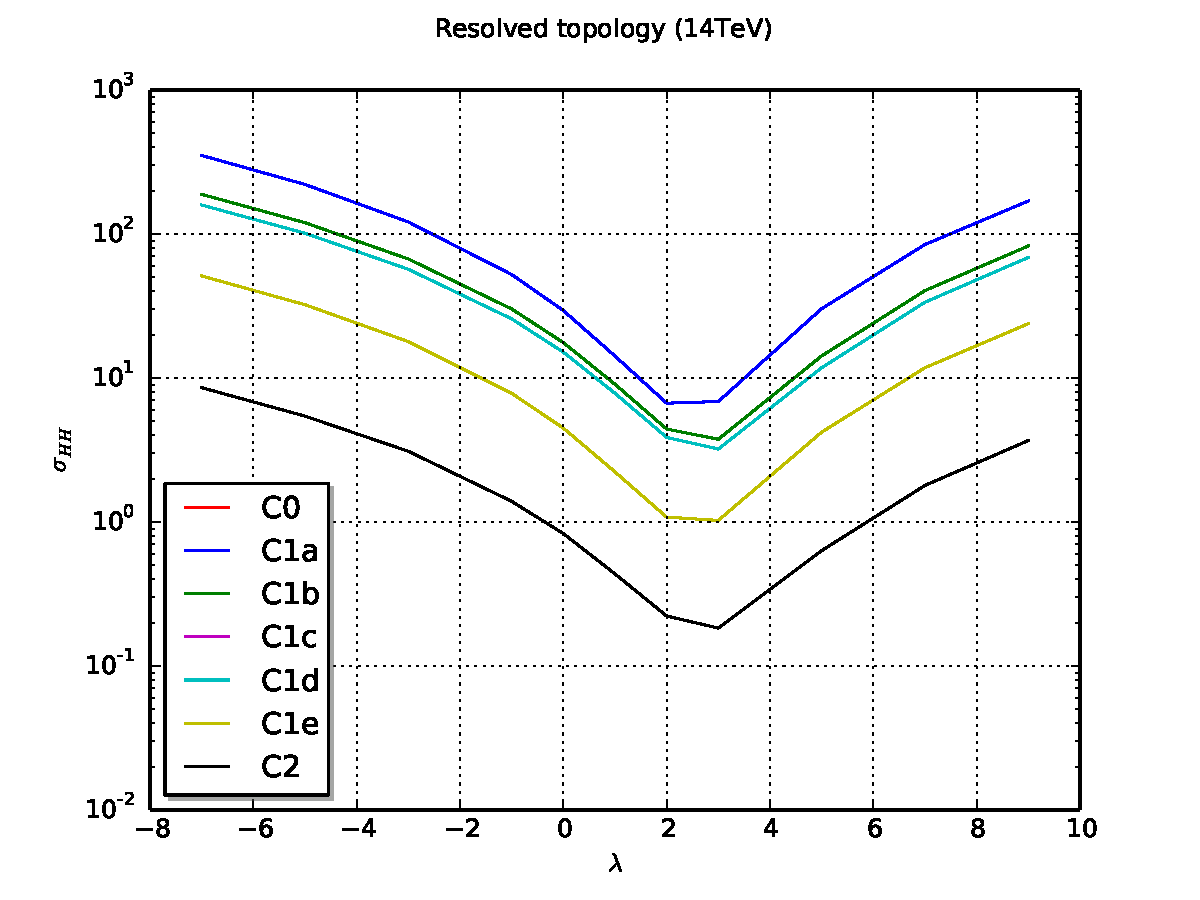
\includegraphics[width=0.45\textwidth]{plots/res_xSec_14TeV.pdf}
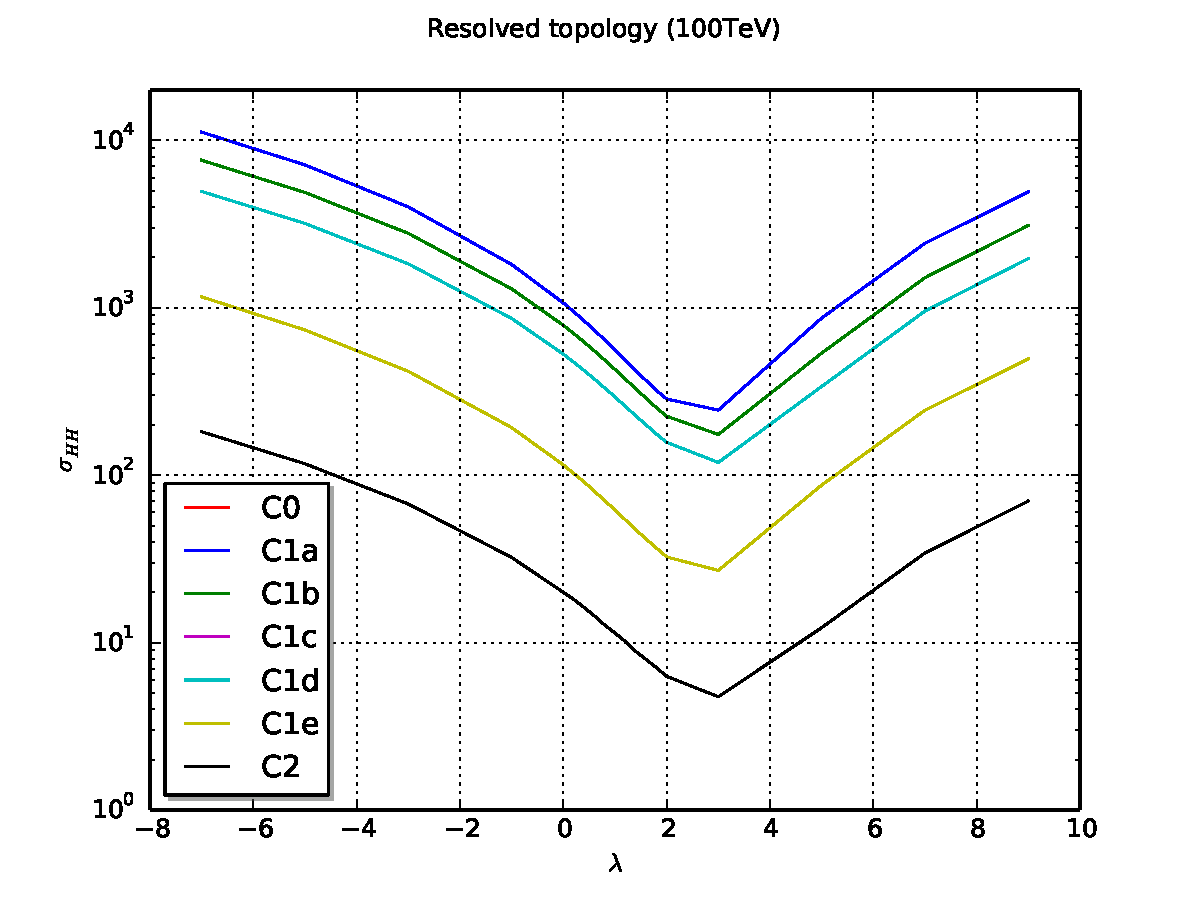
\includegraphics[width=0.45\textwidth]{plots/res_xSec_100TeV.pdf}
\caption{Pre-MVA cross-section variation with $\lambda$ for resolved channel at 14TeV (left) and 100TeV (right).}
\label{fig:resXsec}
\end{center}
\end{figure}

\begin{figure}[htbp]
\begin{center}
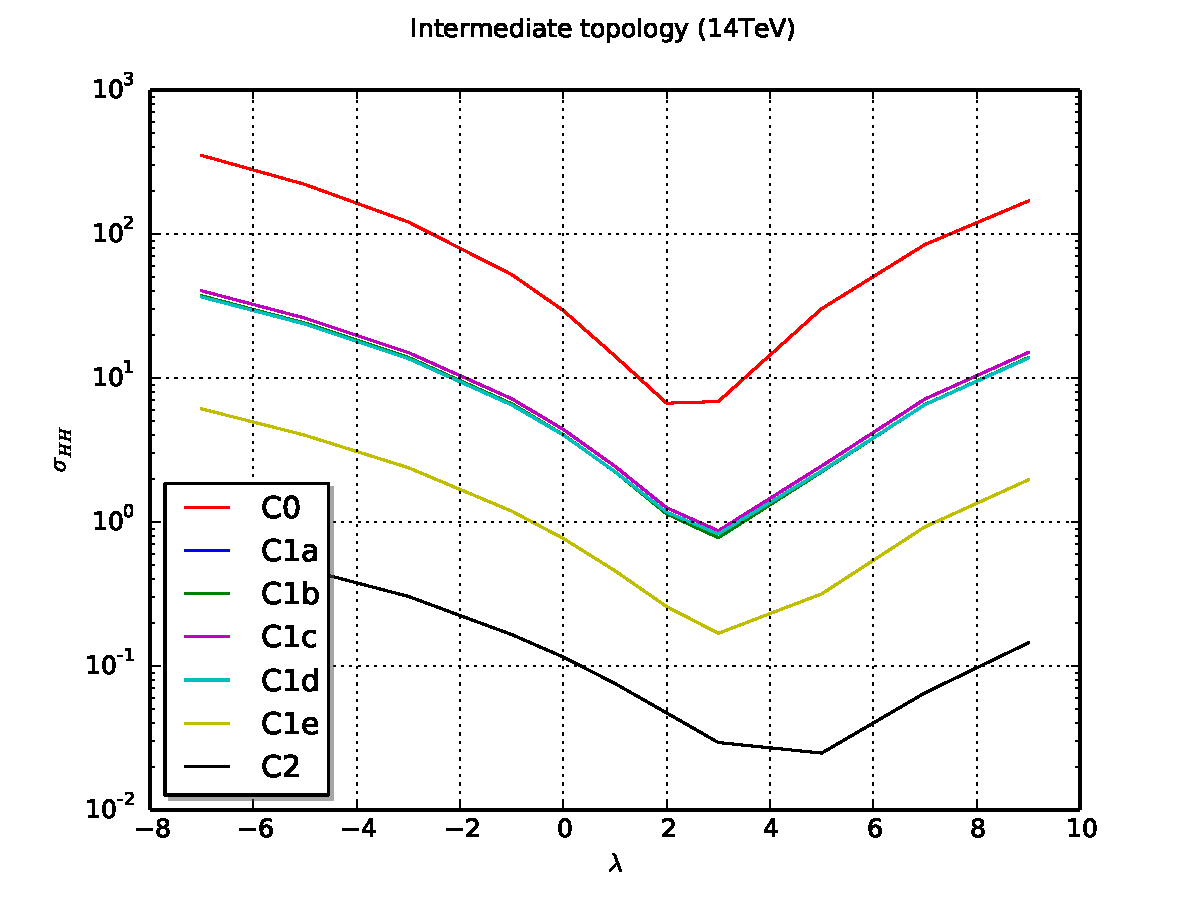
\includegraphics[width=0.45\textwidth]{plots/inter_xSec_14TeV.pdf}
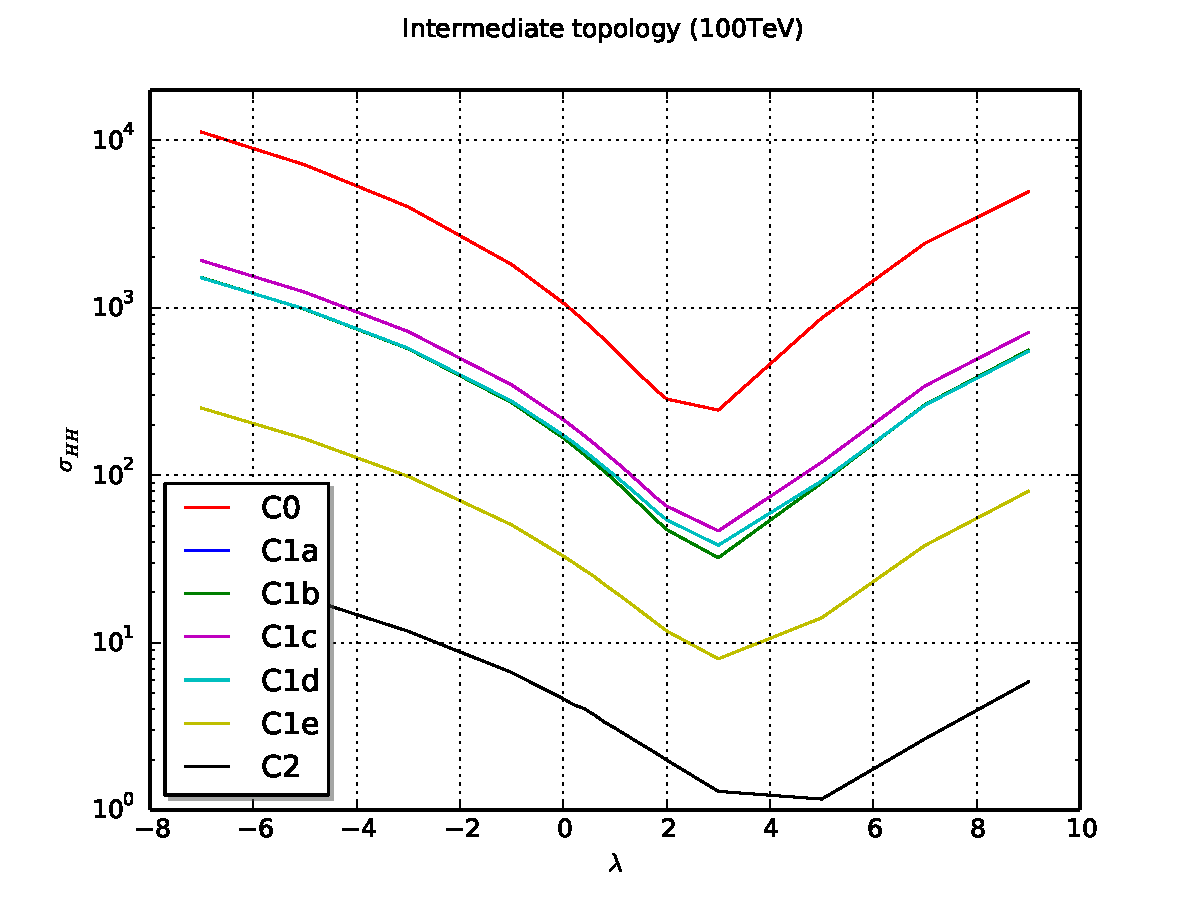
\includegraphics[width=0.45\textwidth]{plots/inter_xSec_100TeV.pdf}
\caption{Pre-MVA cross-section variation with $\lambda$ for intermediate channel at 14TeV (left) and 100TeV (right).}
\label{fig:interXsec}
\end{center}
\end{figure}

\begin{figure}[htbp]
\begin{center}
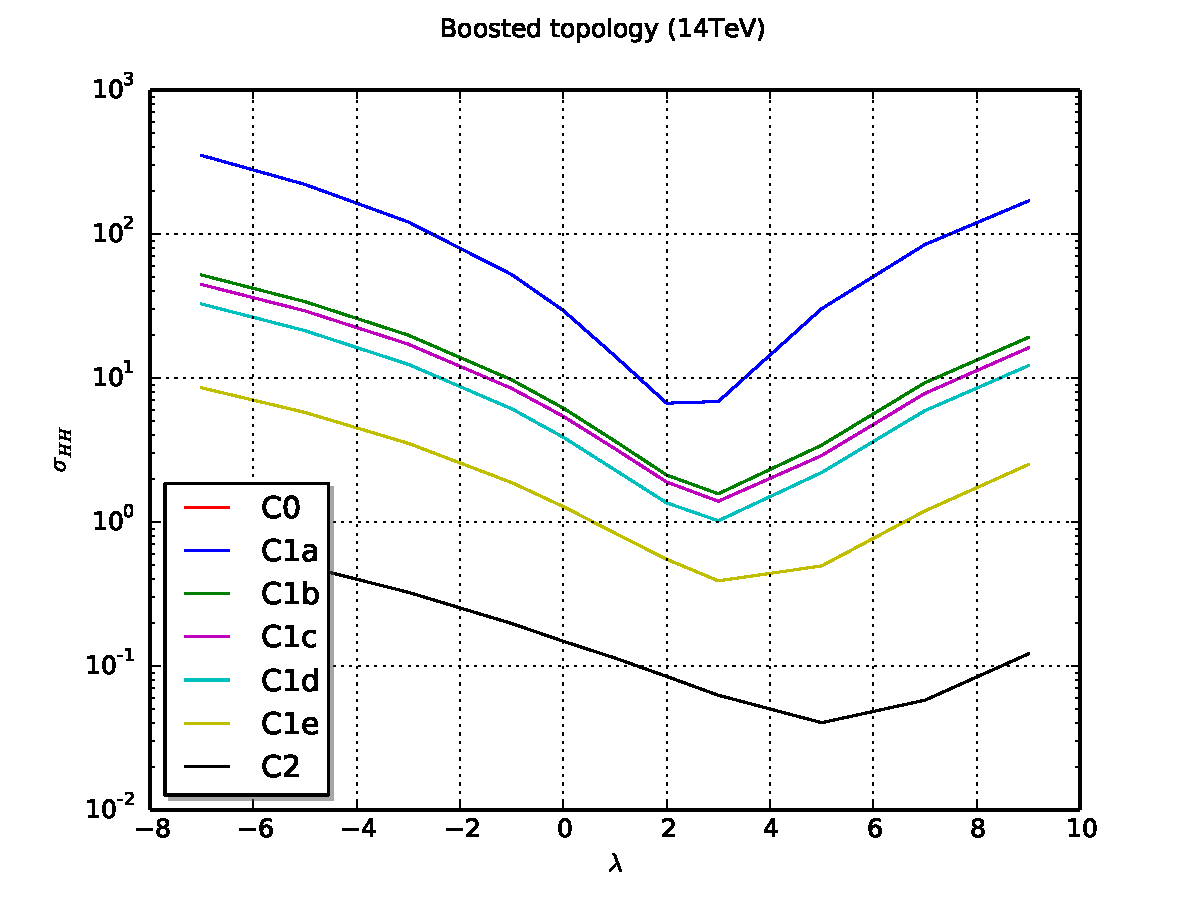
\includegraphics[width=0.45\textwidth]{plots/boost_xSec_14TeV.pdf}
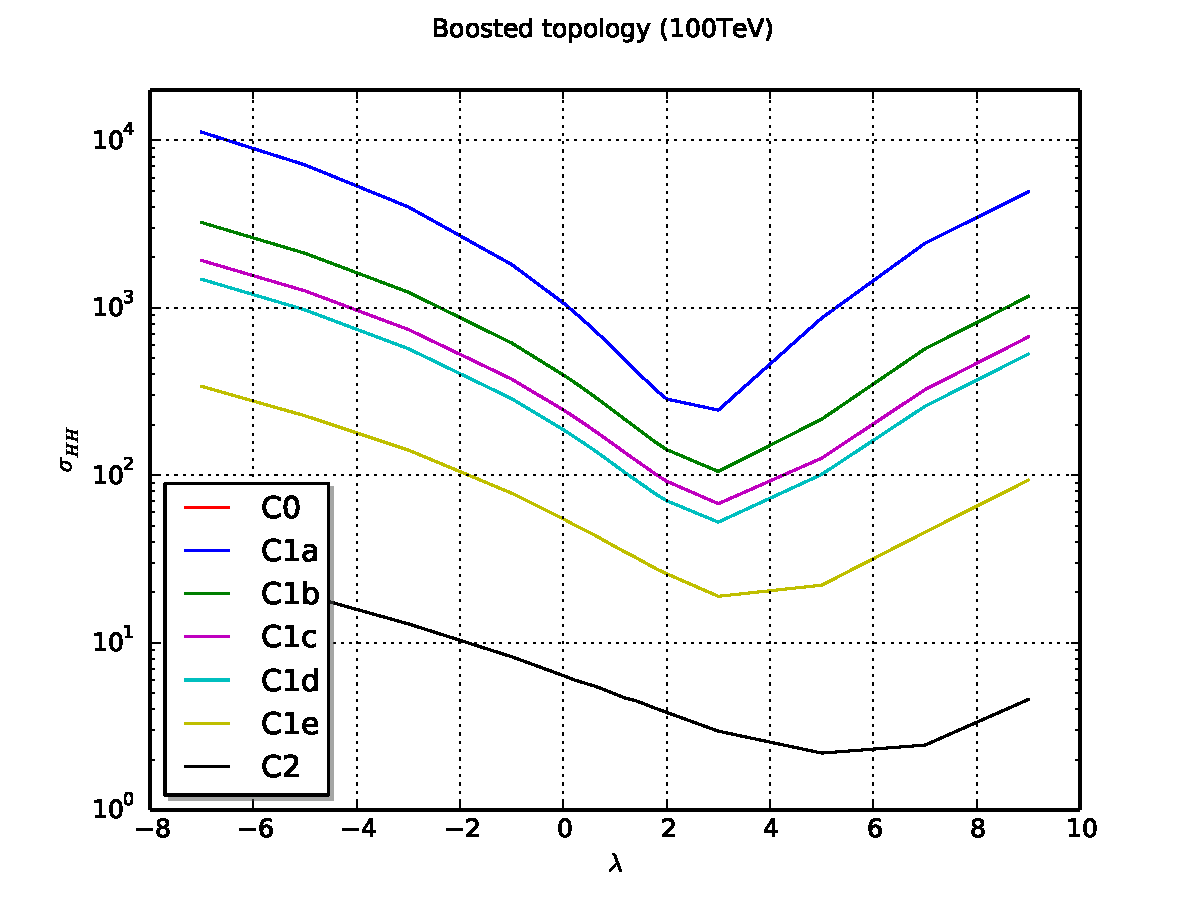
\includegraphics[width=0.45\textwidth]{plots/boost_xSec_100TeV.pdf}
\caption{Pre-MVA cross-section variation with $\lambda$ for boosted channel at 14TeV (left) and 100TeV (right).}
\label{fig:boostXsec}
\end{center}
\end{figure}

\newpage
\section{Trilinear extraction - $\chi2$ profiles}

In this section we show how the trilinear may be extracted under a few assumptions with respect to the systematic uncertainty. Figures are shown for all topologies given a systematic error of zero (Fig. \ref{fig:chi2_0}), 10\% (Fig. \ref{fig:chi2_0_1}) and 100\% (Fig. \ref{fig:chi2_1}).

\begin{figure}[htbp]
\begin{center}
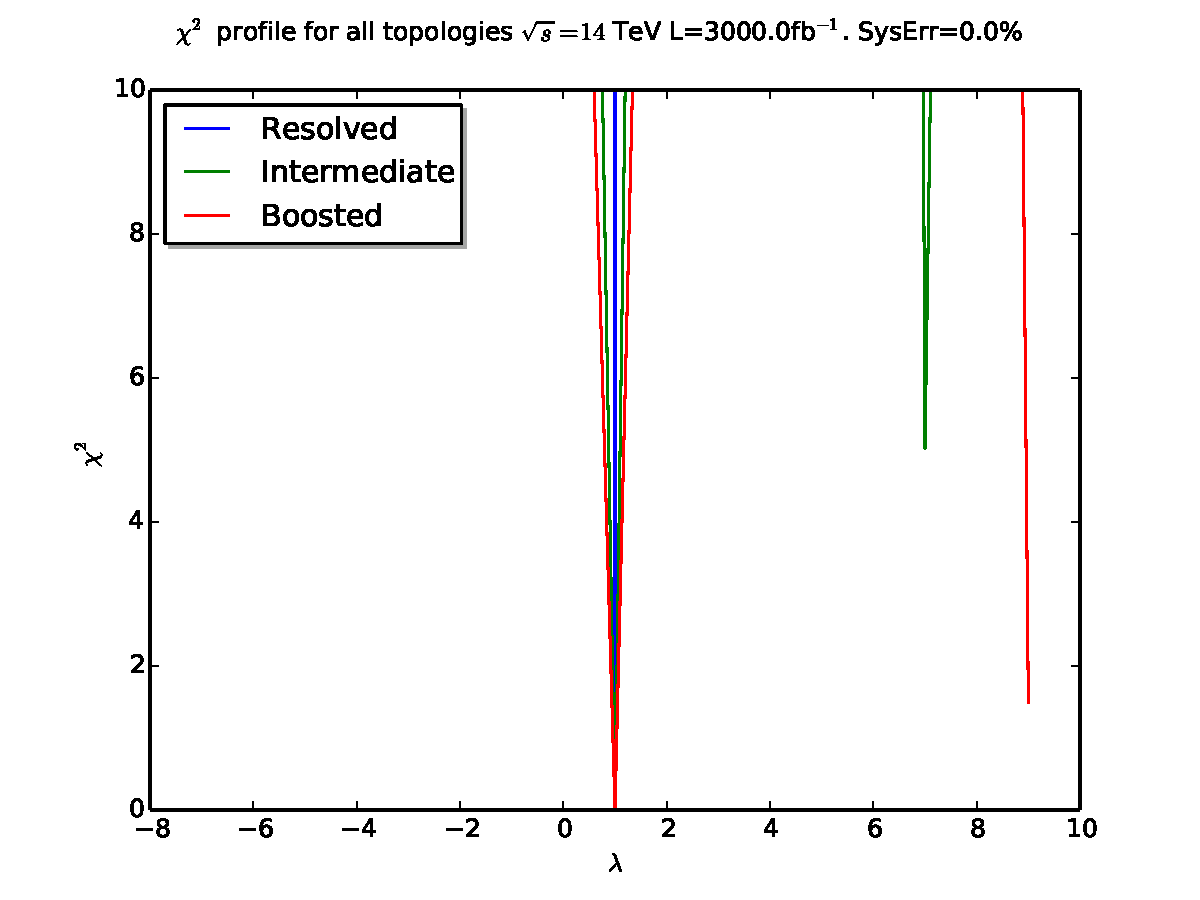
\includegraphics[width=0.45\textwidth]{plots/chi2_14TeV_sys0_0.pdf}
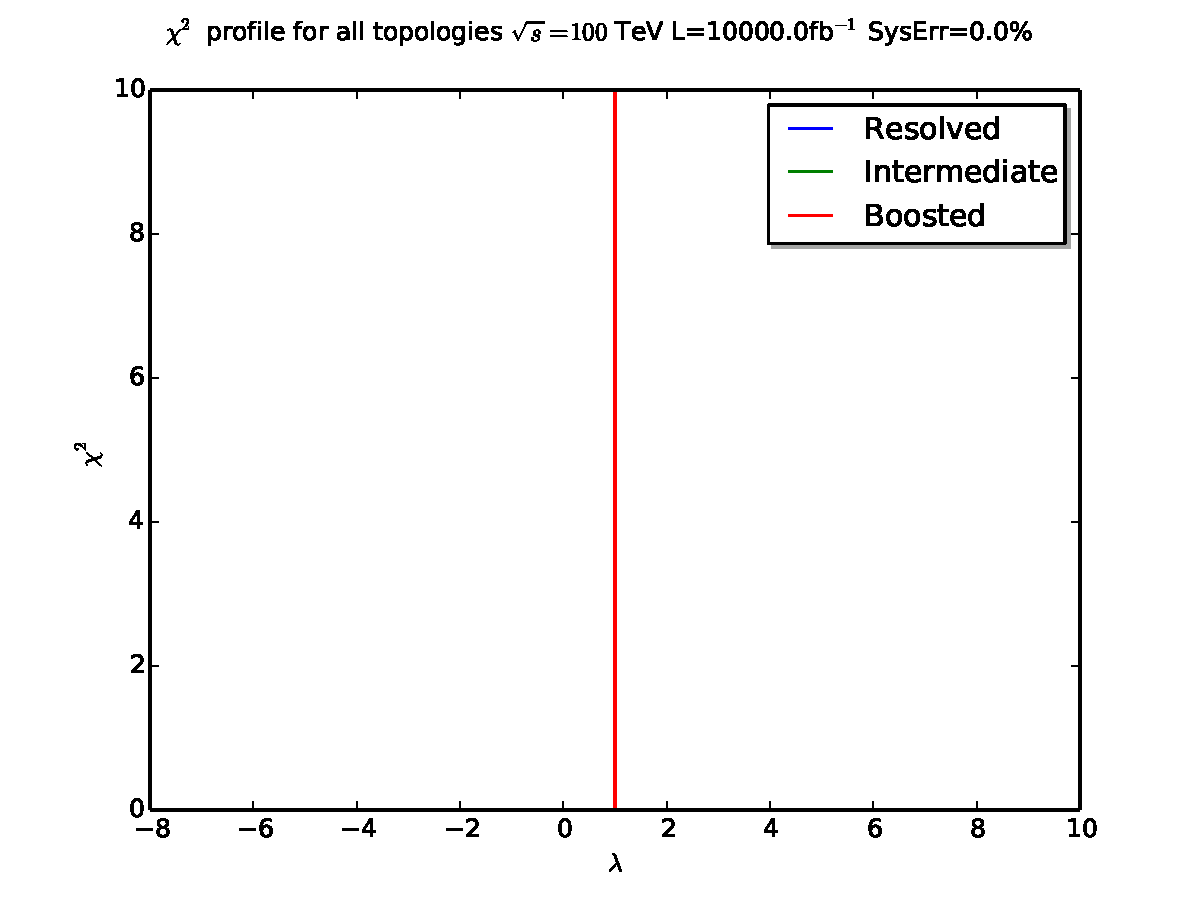
\includegraphics[width=0.45\textwidth]{plots/chi2_100TeV_sys0_0.pdf}
\caption{$\chi^2$ profile for all topologies, 14TeV HL-LHC (left) and 100TeV FCC (right), only statistical error.}
\label{fig:chi2_0}
\end{center}
\end{figure}

\begin{figure}[htbp]
\begin{center}
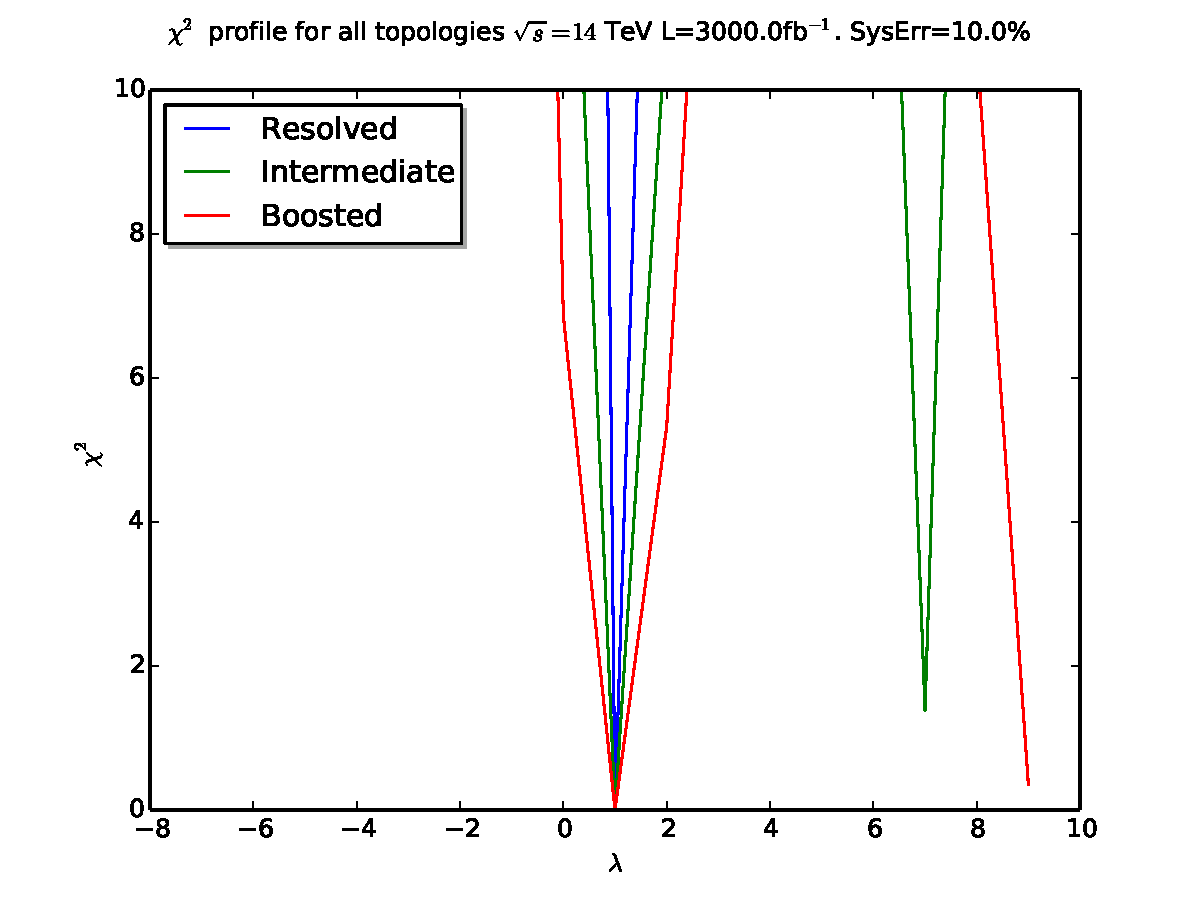
\includegraphics[width=0.45\textwidth]{plots/chi2_14TeV_sys0_1.pdf}
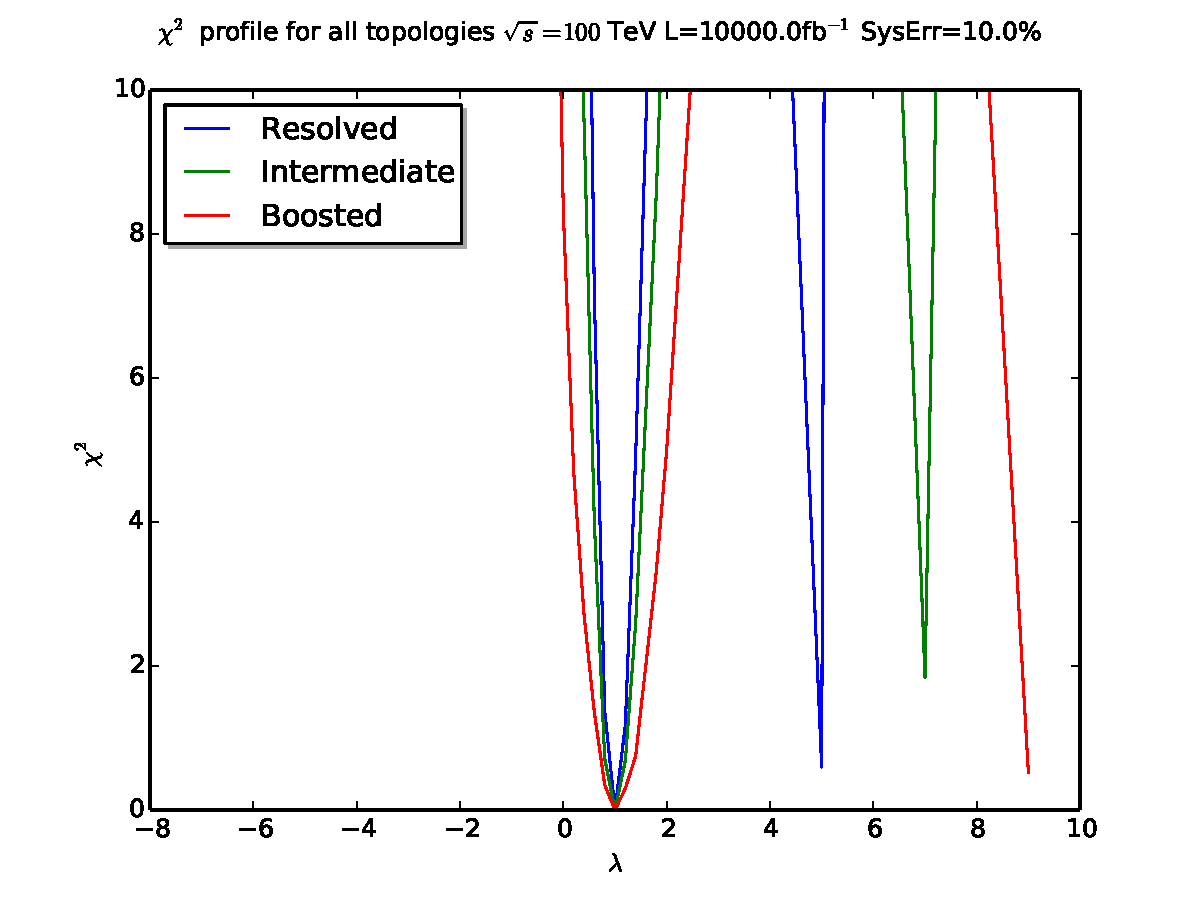
\includegraphics[width=0.45\textwidth]{plots/chi2_100TeV_sys0_1.pdf}
\caption{$\chi^2$ profile for all topologies, 14TeV HL-LHC (left) and 100TeV FCC (right), 10\% systematic error.}
\label{fig:chi2_0_1}
\end{center}
\end{figure}

\begin{figure}[htbp]
\begin{center}
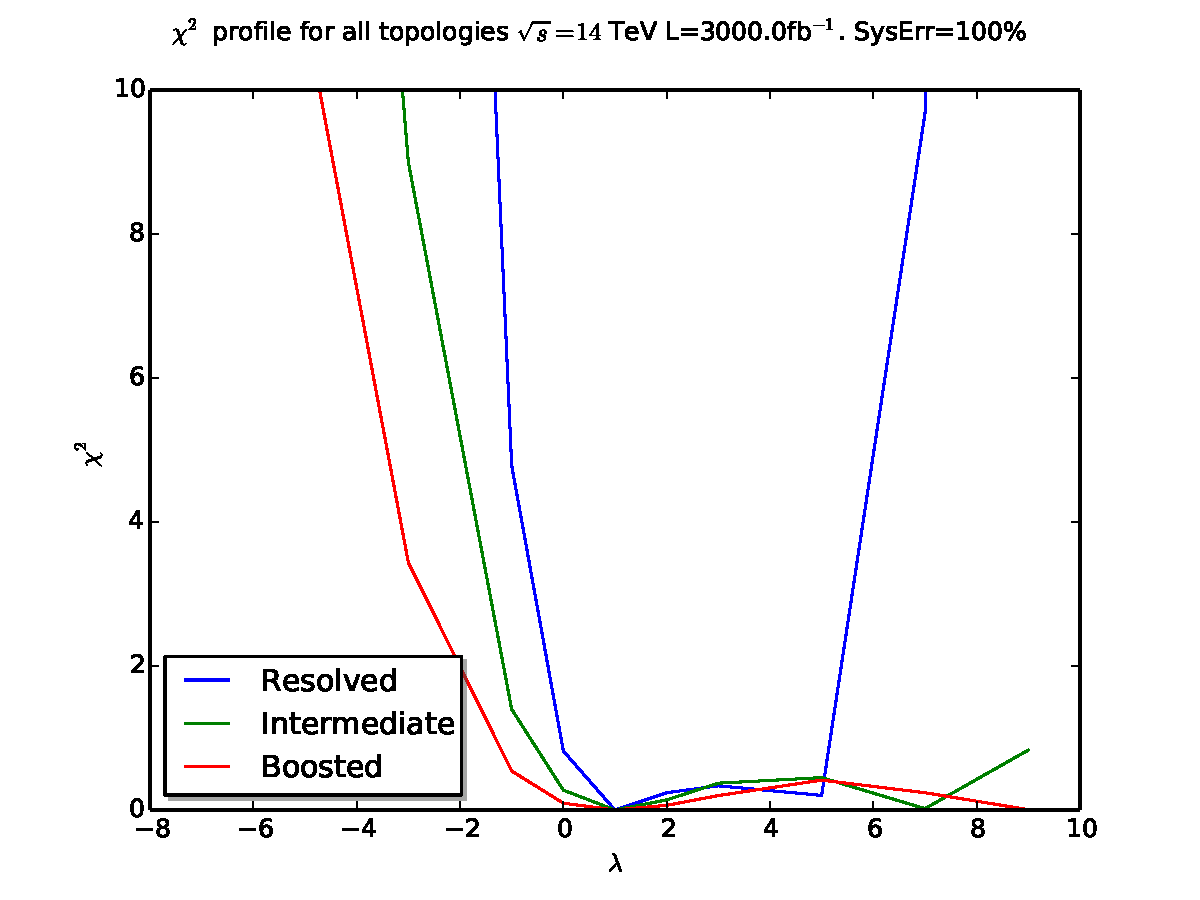
\includegraphics[width=0.45\textwidth]{plots/chi2_14TeV_sys1.pdf}
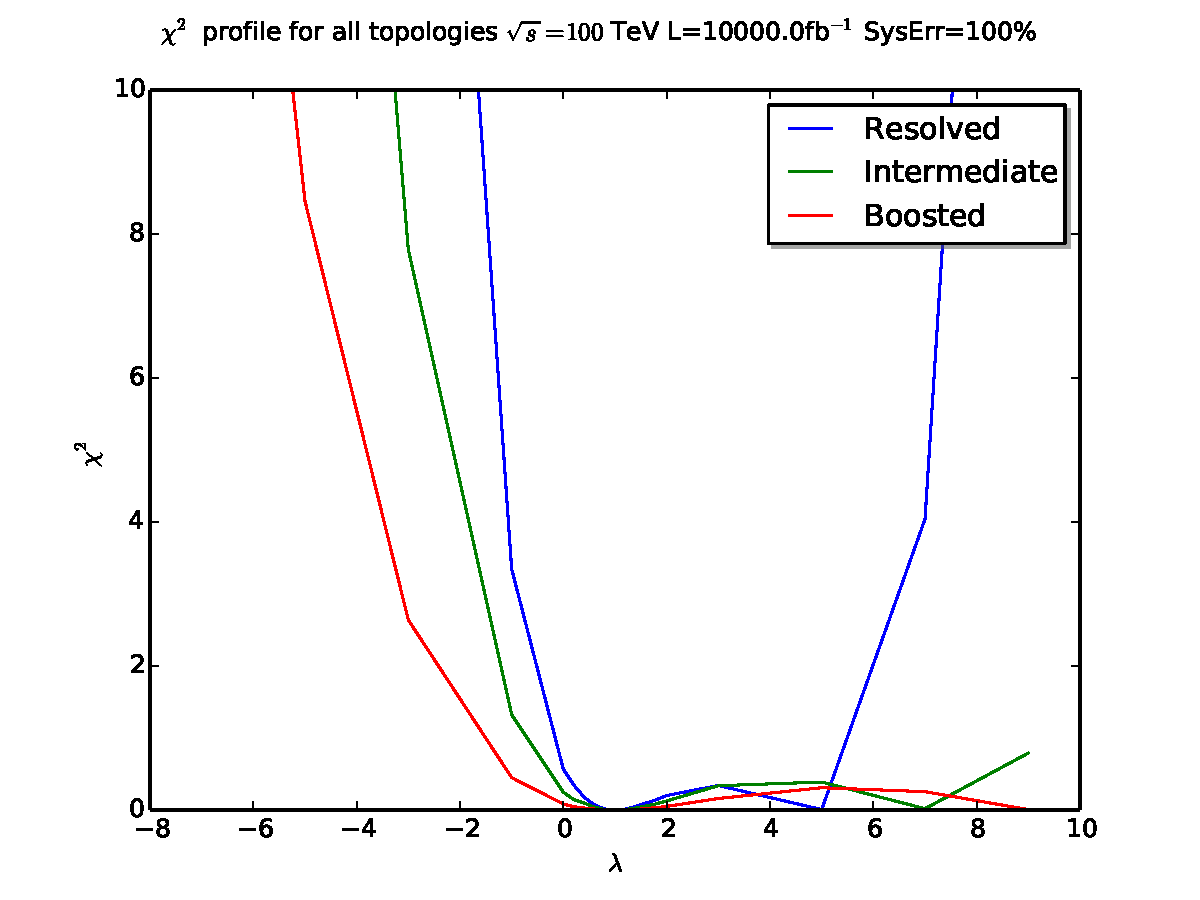
\includegraphics[width=0.45\textwidth]{plots/chi2_100TeV_sys1.pdf}
\caption{$\chi^2$ profile for all topologies, 14TeV HL-LHC (left) and 100TeV FCC (right), 100\% systematic error.}
\label{fig:chi2_1}
\end{center}
\end{figure}

%%%%%%%%%%%%%%%%%%%%%%%%%%%%%%%%%%%%%%%%%%%%%%%%%%%
%%%%%%%%%%%%%%%%%%%%%%%%%%%%%%%%%%%%%%%%%%%%%%%%%%%

\end{document}  